\documentclass[a4paper,10pt]{book}\usepackage{graphicx}
\usepackage{epstopdf}
\epstopdfsetup{update} % only regenerate pdf files when eps file is newer
\usepackage[utf8]{inputenc}
\usepackage{graphicx}
\usepackage{hyperref}
\usepackage{float}
\usepackage{tabularx}
\usepackage{pdfpages}

\restylefloat{table}
% Title Page
\title{Exam Report Communication Networks II}
\author{Daniel Ploeger, Nina Piontek}

\begin{document}
\maketitle
\tableofcontents



\chapter{Network Description}
Because of a construction site near Channel 4 which might accidentally damage the cables 
used for internet connection,
a point-to-point radio link should be implemented to ensure network connection.
In the following, the new network configuration as depicted in \ref{fig:network} will be evaluated.
\begin{figure}[!ht]
  \centering
    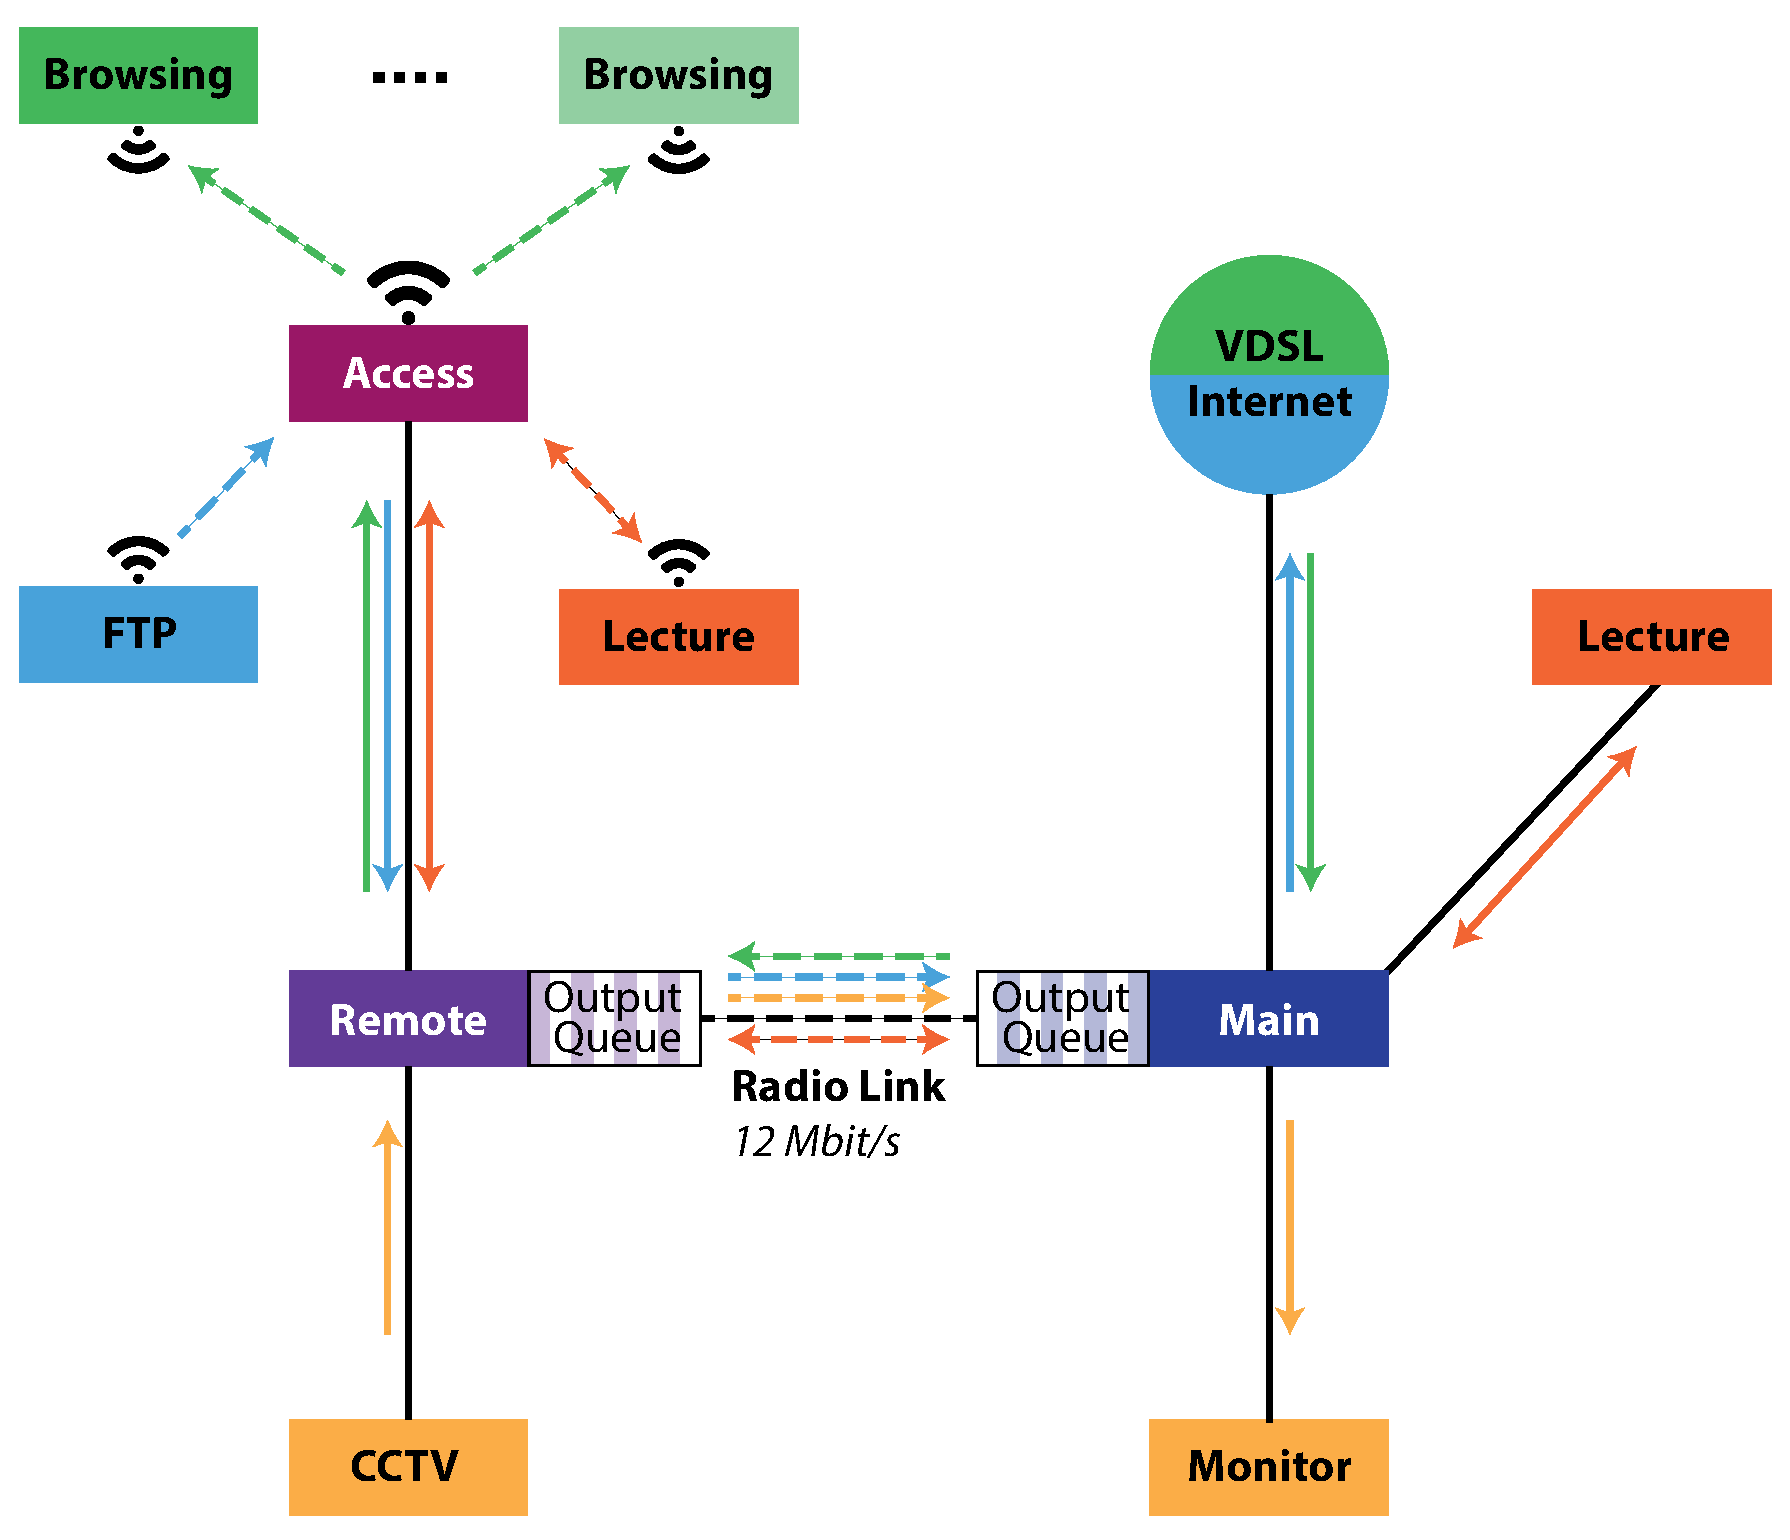
\includegraphics[width=0.9\textwidth]{graphics-03.eps}
    \label{fig:network}
    \caption{University Network}
\end{figure}

\section{General Discription of the Main Components of the Network}
The network core is a set up with 2 Routers, Main Router (M) and Remote Router (R), connected with a Point-to-Point Link. 
Towards the Main Router the Porters Office' Computer and the Computer of the Professor giving the remote Lecture are connected.
The Main Router is the Gateway for the shared Internet Connection of the University.

Towards the Remote Router the Access Point for WLAN and the Security Camera are connected.
The Access Point provides Wireless Lan for Students at Channel 4. The Computer for the Video Lecture at Channel 4 
is connected via WLAN as well.



\section{Network Services and Requirements}

In this set up the Network performance regarding the Video Lecture is evaluated with the following Services in
use:\\
\begin{enumerate}
 \item WLAN for Webbrowsing
 \item FTP Service for Uploading a file to a Server in the Internet (used by one Student) 
 \item Video Lecture streamed in both directions from the Main Campus to Channel 4
 \item Security Camera streaming from Channel 4 to the Porters Office  at the Main Campus
\end{enumerate}

The network should provide a certain Quality of Service for the Video Lecture and the Security Camera.
The Criteria are:\\
\begin{enumerate}
 \item The Video Data should not take more than 100ms to be delivered to the destination in both directions.
 \item There should only be a loss of data at most of 5$ \% $
\end{enumerate}

\chapter{Network Modeling}
\section{General Assumptions on the Model}
Since the overall Goal is to evaluate the network performance regarding the Qos during the Video Lecture, we will assume an assessment period
of around 90 minutes. The WLAN at Channel 4 will in general be used by the Students, which surf the Web during the Video Lecture and the Student 
who uploads a file. Optional the Camera will be turned on or switched off to evaluate the networks behavior with and without the additional
traffic load.
\subsection{HTTP Traffic}
In order to model the student web browsing behaviour in 
a meaningful way, captured browsing statistics have been provided by the computer center in a trace file. 
This chapter shortly explains the statistical behaviour behind the given HTTP 
requests and responses. The response sample traces (download statistcs) are widely 
distributed in the range of less than 500 Bytes up to more than 4 Mbyte 
(see figure XXX top).

Distribution fitting analysis shows that the statistical behaviour if
 partitioned in a smaller number of bins roughly behaves like a negative 
exponential distribution with a mean value of 0.789 Mbyte (see figure XXX center). 
The phrase "roughly" means that while the statistical goodness of fit tests accepts
 this distribution, the actual data has an overweight of small messages compared to
 the expected values (see figure XXX bottom). An exponential distribution with the
 mean of 0.789 Mbyte is used in this report for simulation nonetheless. 
This is a conservative approach and guarantees an upper bound in the distribution:
 if the actual browsing behaviour uses smaller HTTP responses with a slightly higher
 probability, the QoS assumptions from the following chapters are going to be met 
in practice as well.
\subsection{Network Behaviour - General Expectations}

\begin{minipage}[H]{\textwidth} 
\begin{tabular}{|l|l|l|l|l|}
\cline{1-4}
 Link & Data Rate  & Downlink  & Uplink  \\ \cline{1-4}
 WLAN & 54Mbit/s  & HTTP, Video Lecture & FTP,Video Lecture \\ \cline{1-4}
 Access Point $\leftrightarrow$ Remote Router & 100Mbit/s  &HTTP, Video Lecture& FTP  \\ \cline{1-4}
 Camera $\leftrightarrow$ Remote Router & 100Mbit/s  & - & Camera\\ \cline{1-4}
 Remote Router$\leftrightarrow$Main Router&12 Mbit/s&HTTP,Video Lecture& FTP, \\ 
 & & & Video Lecture,Camera \\ \cline{1-4}
 Main Router$\leftrightarrow $ Porters Office &Ideal Connection &Camera& - \\ \cline{1-4}
 Main Router$\leftrightarrow $ Professor & -  &Video Lecture&Video Lecture \\ \cline{1-4}
 Main Router$\leftrightarrow $ Internet &100Mbit/s &HTTP& FTP \\ \cline{1-4}
\end{tabular}
\end{minipage}

The point-to-point radio link between remote and main router has a data rate 
of 12 Mbit/s and by this is the weakest single link within the proposed network. 
All other connection speeds are multiples of this data rate. Since all data has 
to pass this link, for this theoretical behaviour analysis it is considered to 
be the network bottleneck.

The network contains several applications which have their main impact either
upload connection in the other direction. The respective opposite direction of an
 application may be neglected, since it mainly consists of very small messages for connection management or empty network packets. For 
 this reason, theoretical down- and upload utilization is examined independently from each other in this chapter. 

The only exception is the video conference, which utilizes both, up- and download 
equally. The video stream consumes 280 kbit/s for transmission of 1388 Bytes of 
payload plus 12 Byte RTP protocol headers. It does this every 40 ms and in both 
directions.

\section{Upload Connection, Remote to Main Router}

Aside from the video conference which uses 280 kbit/s, two more applications make use of the upload direction. Firstly, the CCTV camera 
sends 10 KB every 40 ms, which adds up to 2,000 kbit/s. The second application is the FTP upload. It tries to maximize 
network utilization and should therefore consume the biggest part of the remaining 9,720 kbit/s of the 12,000 kbit/s data rate 
(see figure XXY left).

\section{Download Connection, Main to Remote Router}

Apart from the video conference, the only application which makes use of the download direction is the web browsing. 
As stated before, web browsing is modelled as the download of files with a exponentially distributed size with a mean of 
0,789 Mbyte (see chapter section HTTPTRaffic). The client's assumption states that a web browsing user waits a certain time before he 
downloads the next file. The waiting time is assumed to be exponentially distributed with a mean of 15 seconds. 
This leads to an expected average data rate of 420.8 kbit/s per user. Therefore, if all users download in a well-distributed way, 
up to 27 users are able to browse simultaneously via the network connection (see figure XXY right).


\chapter{Simulation Results}
\section{Without Camera\\ {\large Nina Piontek}}

Since the default configuration for the Links is full-duplex, we evaluate the performance of the Uplink and the Downlink independently.
\section{Expectations on Uplink}
When the Camera is turned off, the Point-to-Point Link to the Main Campus is shared between the FTP Upload and the Video Lecture (Video Conference).
Since the Video Conference is sending with a constant Data Rate of 280kbit/s, the remaining 
11,72 Mbit/s can be used by the FTP Upload.
\begin{figure}[!ht]
  \centering
    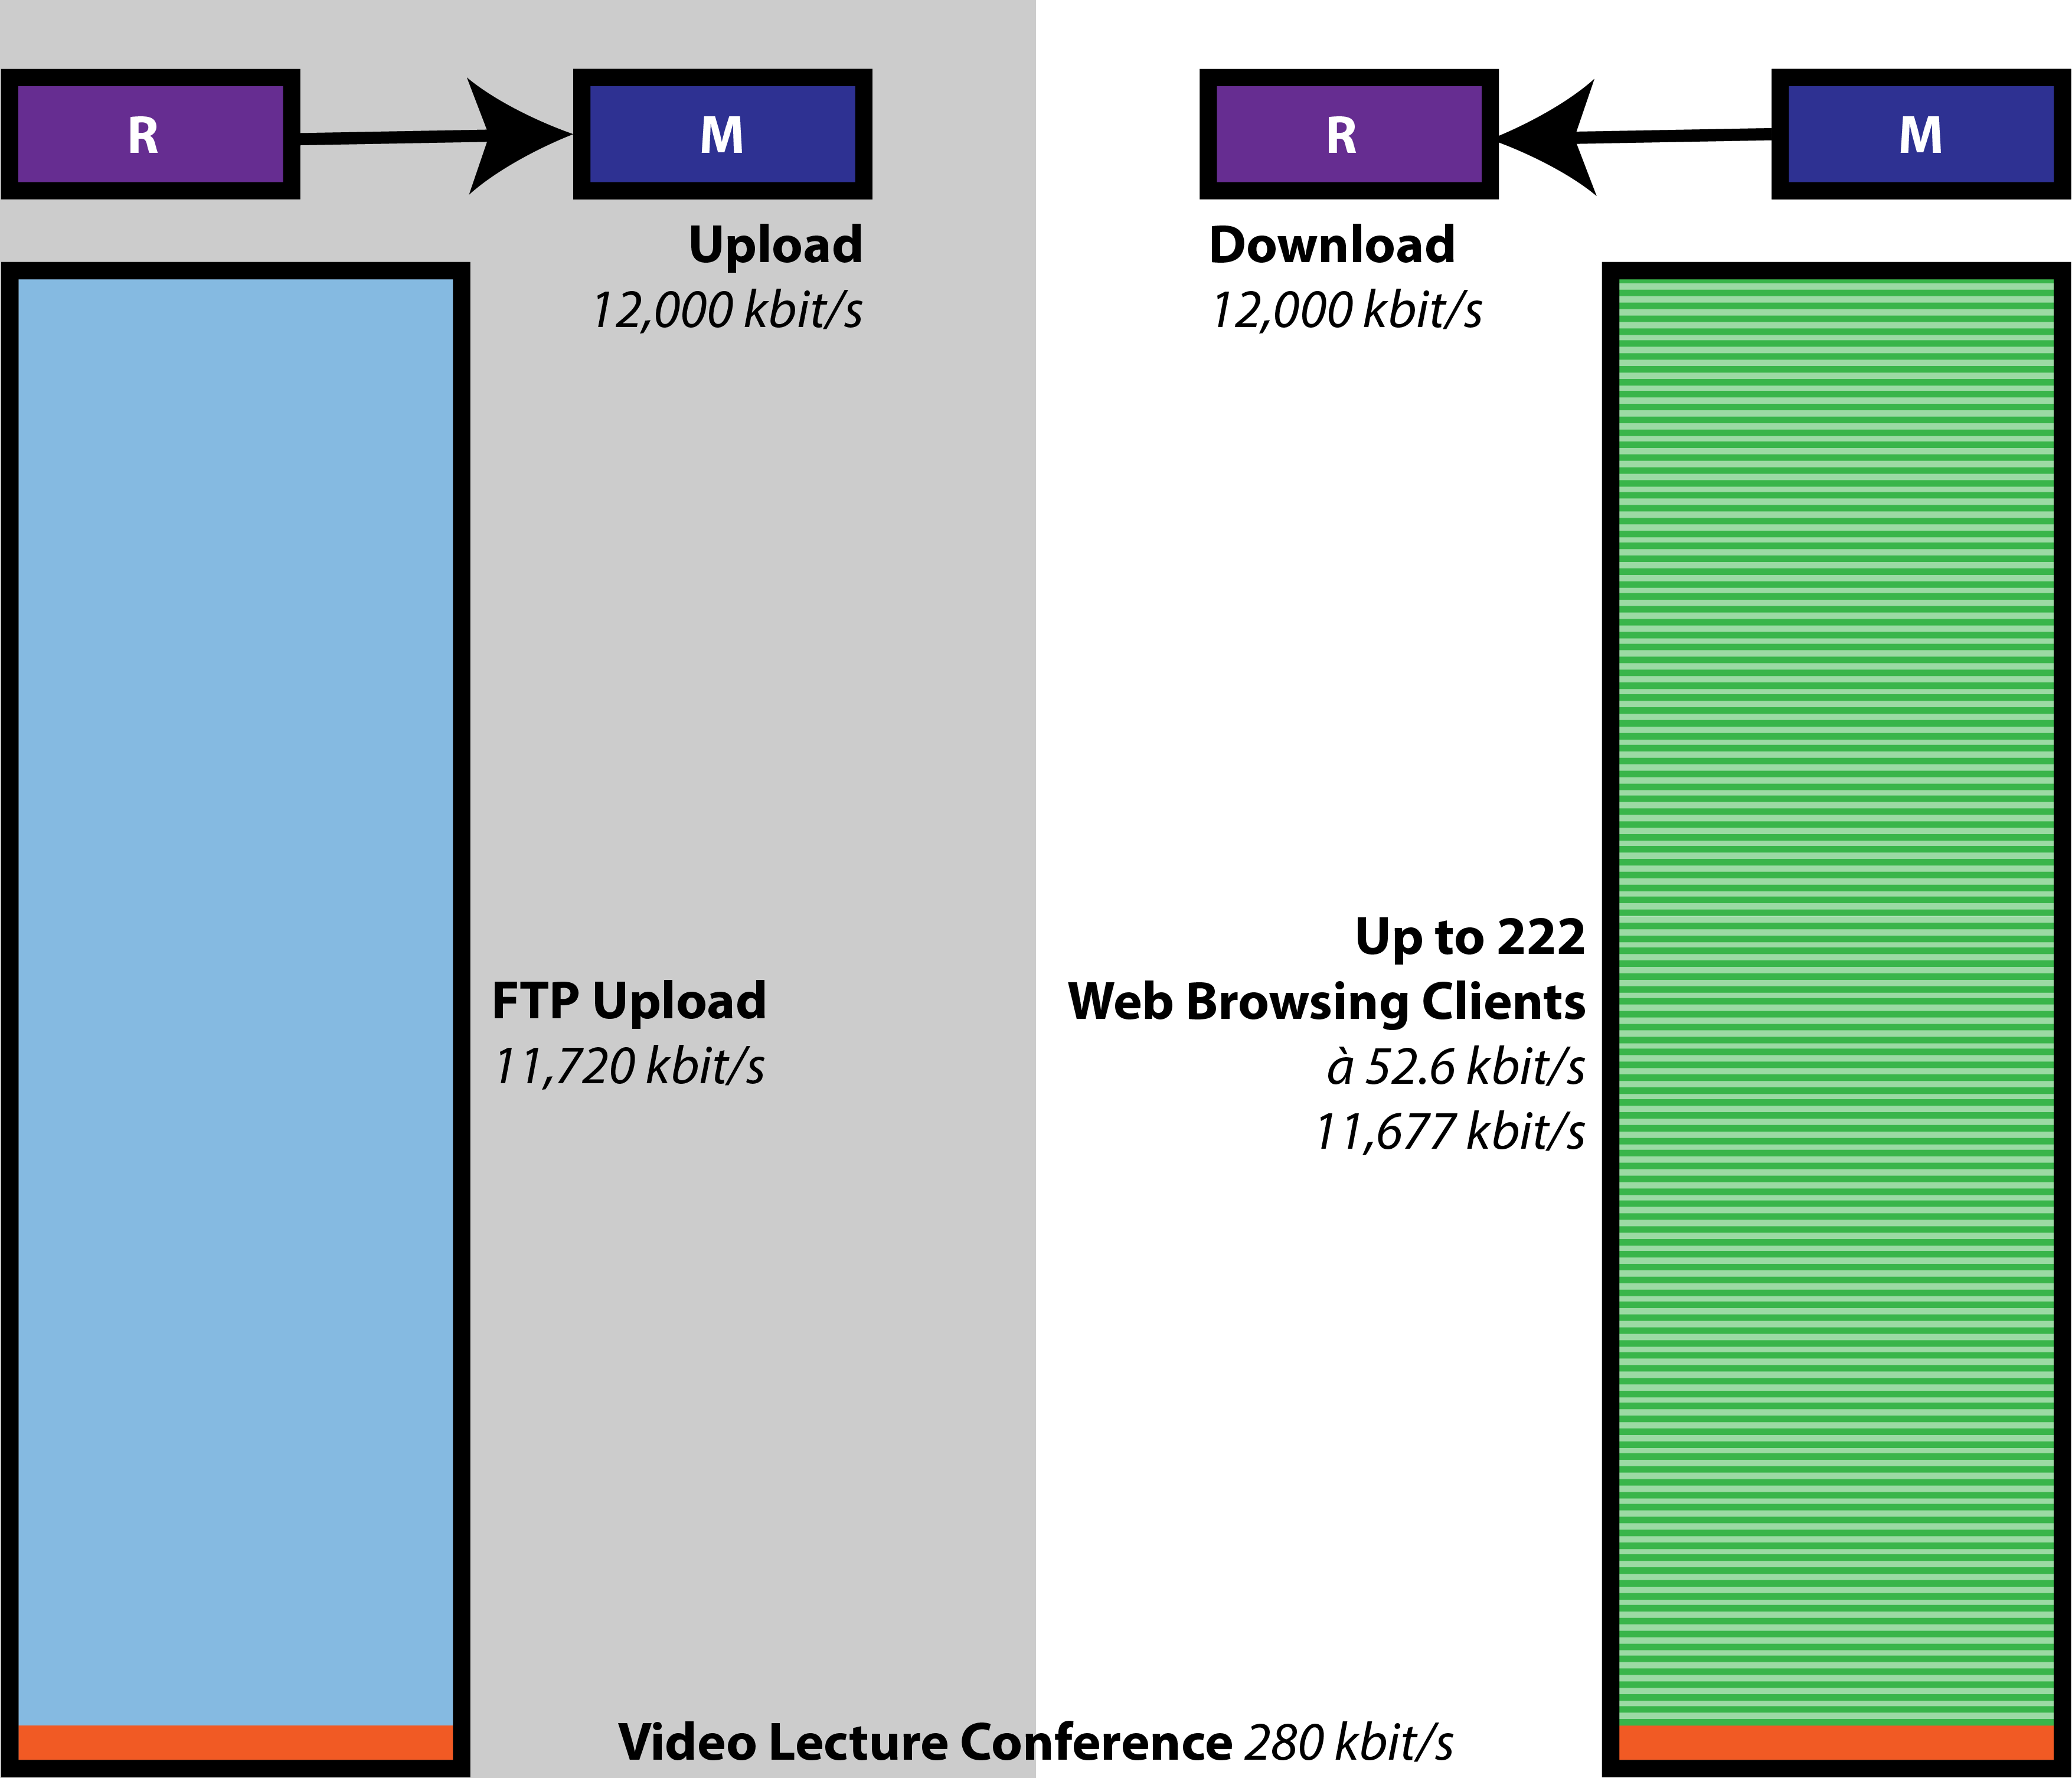
\includegraphics[width=0.9\textwidth]{graphics-02.png}
    \label{fig:g2}
    \caption{Utilization of the Radio Link without the Security Camera streaming}
\end{figure}

\section{Expecations on Downlink}

On the Downlink the Data Rate of 12Mbit/s is shared between the Students browsing the Web (HTTP Service) and the Video Lecture (Video Conference).
Since the Downlink is utilized by the Video Lecture by 280kbit/s , the remaining 11,7Mbit/s 
can be theoretically used by the HTTP Service.



\chapter{Expectations on the Network Behavior - with Camera}





\begin{figure}[!ht]
  \centering
    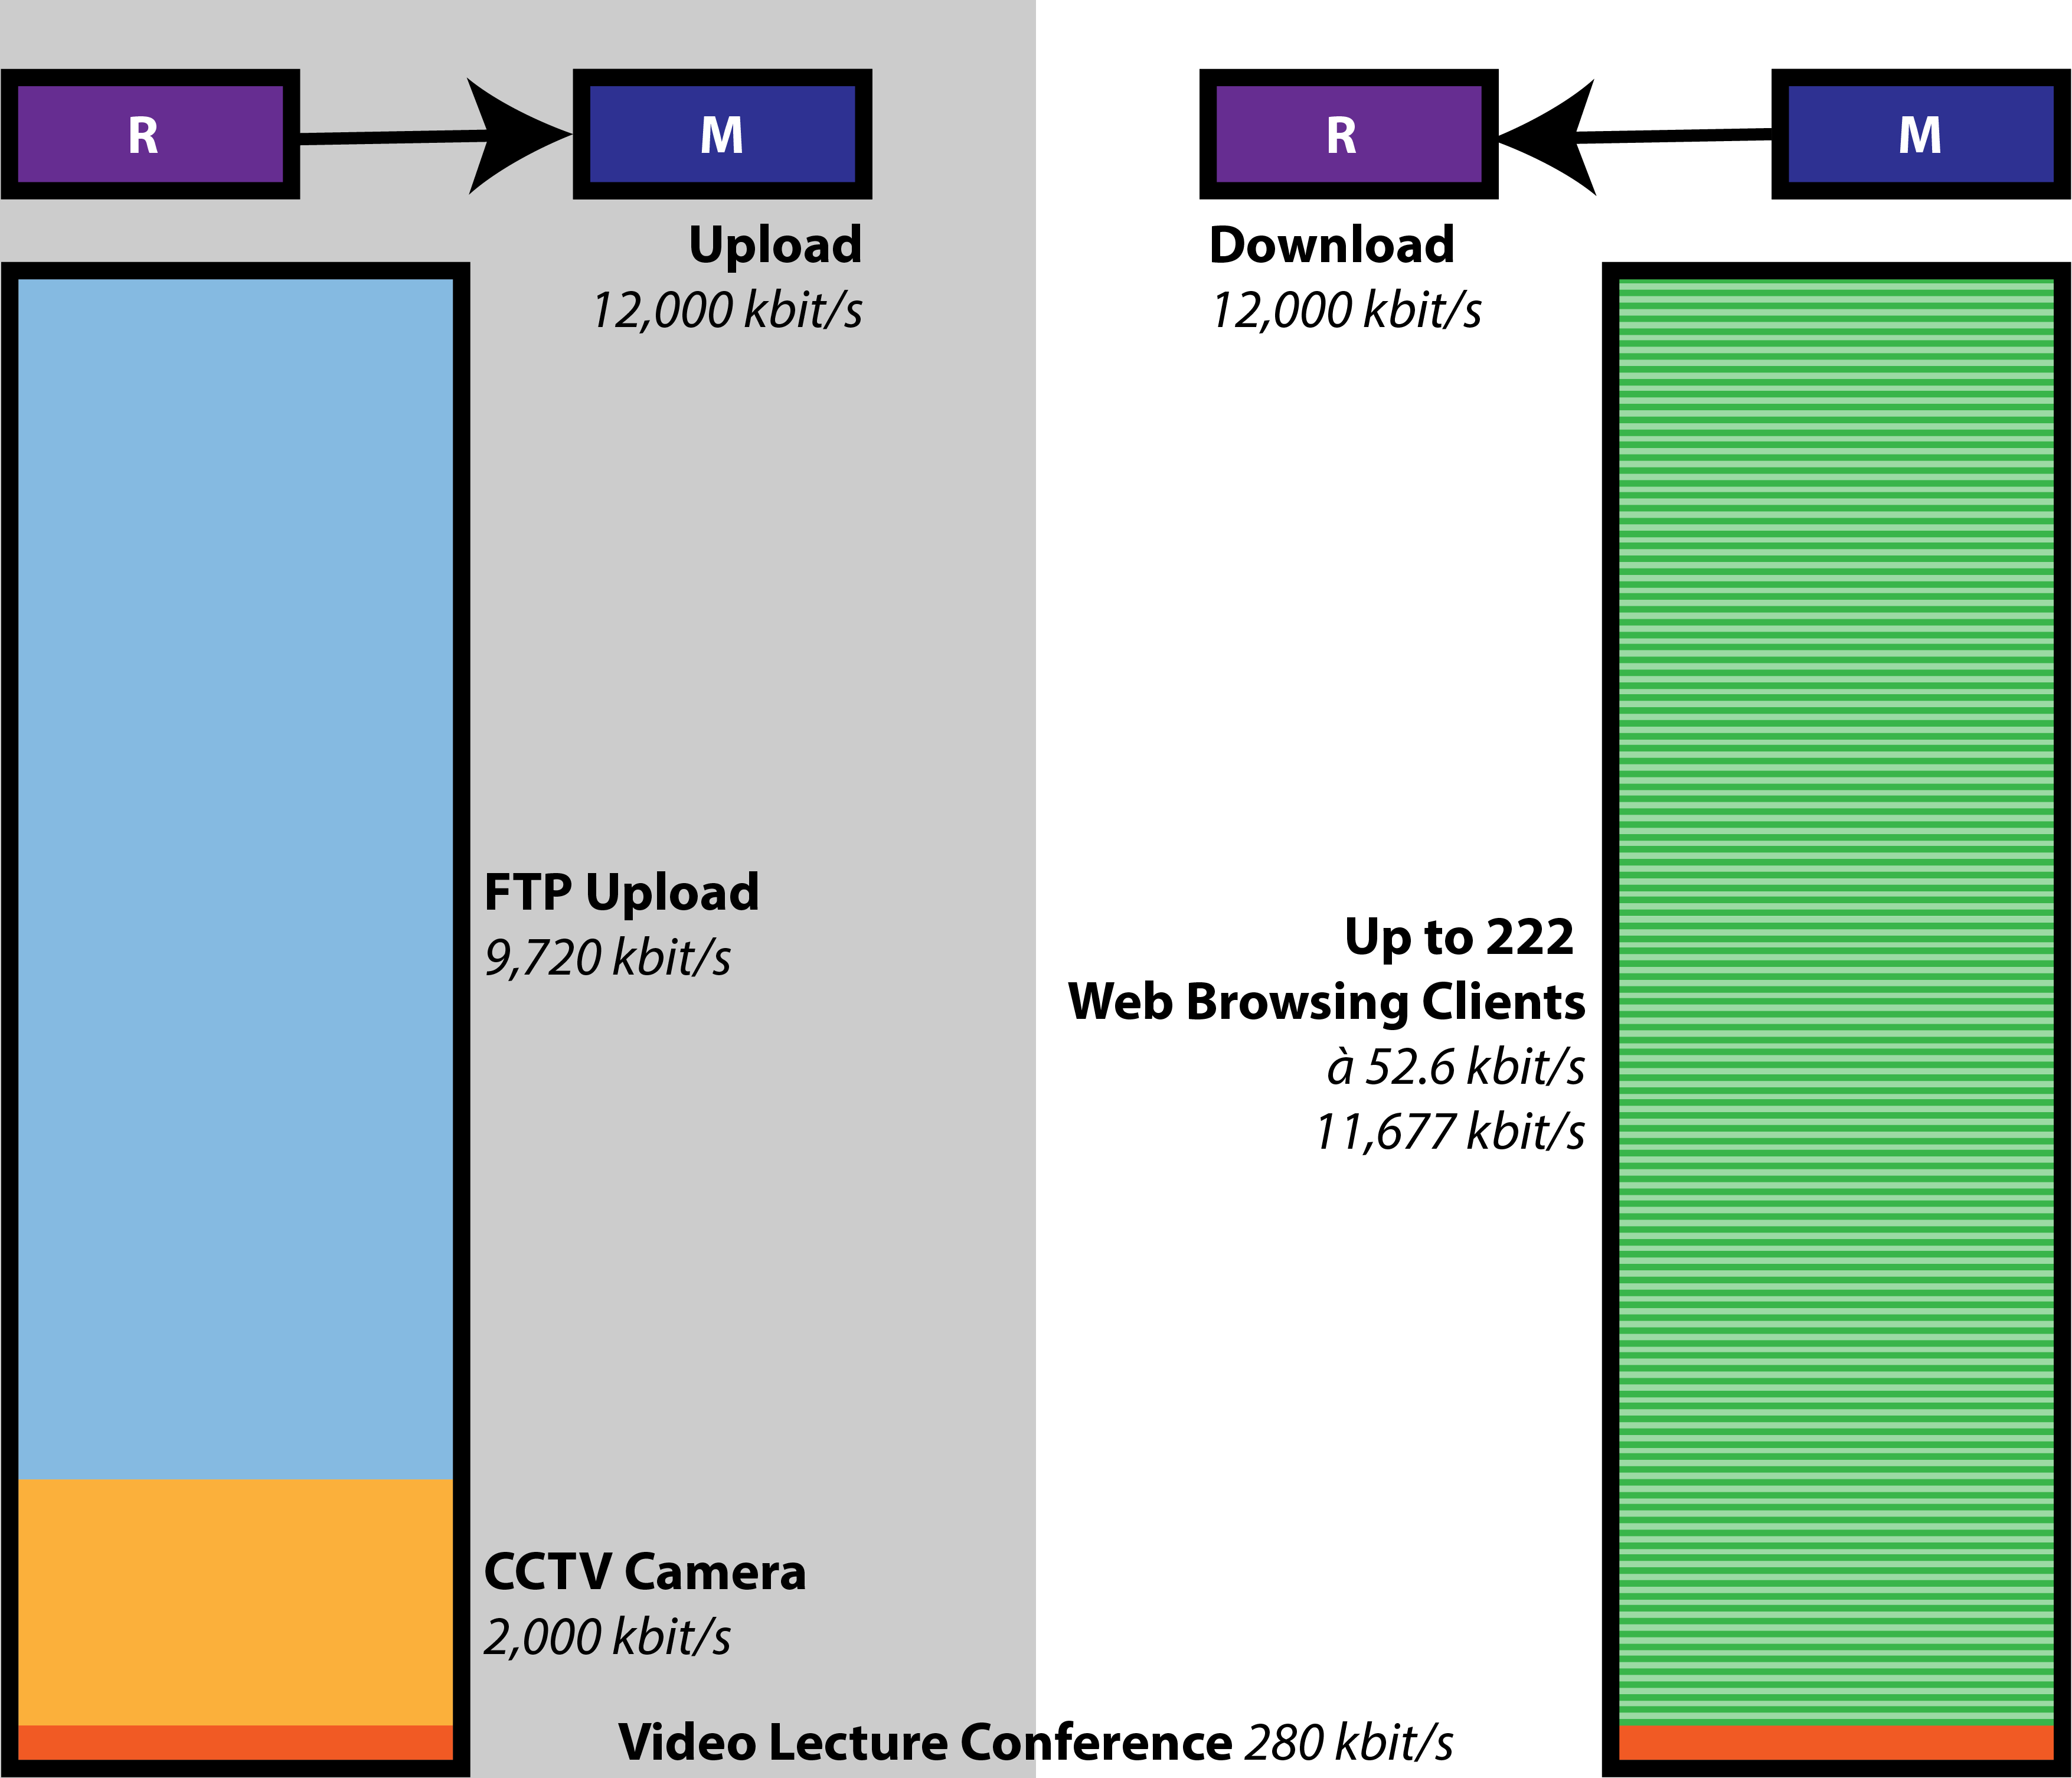
\includegraphics[width=0.9\textwidth]{graphics-01.png}
    \label{fig:g1}
    \caption{Utilization of the Radio Link with the Security Camera streaming}
\end{figure}










% The Network should be able to provide good quality of service regarding a situation where the traffic load is determined by the following 
% services:
% \begin{enumerate}
%  \item Remote Video Lecture
%  \item Surveillance of the Entrance
%  \item WebBrowsing
%  
% \end{enumerate}
% 
% 
% The Network should be able to provide good quality of service regarding a remote Video Lecture. The Network performance will be evaluated 
% regarding 
% 
% 
% 
% 
% 
% 
% Key Apects are:
% \begin{enumerate}
%  \item How many User can surf the Web 
% \end{enumerate}
% 
% The considered situation is determined by the following assumptions:
% 
% \begin{enumerate}
%  \item A
% \end{enumerate}


% 
% 
% 
% \chapter{HTTP Service}
% average download rate of the http client
% how many students can use the web while the file is uploaded, the camera is streaming and the professor is giving the lecture, so that the
% Qos  requirements ( delay, loss rate ) are still met?
% \section{Expectations and theoretical Justification}
% \section{Video Conference}
% How do  the other apps influence the call.
% Is it required to Pause the CCTV camera during the video lecture?
% Is the Radio Link sufficient for the Video Call? Improvements of the Qos?
% \subsection{Influence of CCTV Camera on Video Conference}
% Where is the main bootleneck of the network, when the CCTV camera is turned on?
% Where is the main bootleneck of the network, when the CCTV camera is turned off?
% \subsubsection{Expectations and theoretical Justification}
% Confidence Intervals 
% \chapter{Simulation Results and Interpretation regarding the Expectations}
% \section{Radio Link}
% Is the radio link sufficient for all services to meet te Qos of all Apps?
% \subsection{Expectations and theoretical Justification}
% Confidence Intervals 
% \subsection{Simulation Results and Interpretation regarding the Expectations}
% 
% \section{FTP Service}
% average data rate of the ftp upload
% \subsection{Expectations and theoretical Justification}
% Confidence Intervals 
% \subsection{Simulation Results and Interpretation regarding the Expectations}

\end{document}          
